% Version 6: Figure
\documentclass[11pt]{beamer}

\usetheme{Frankfurt}
\setbeamertemplate{navigation symbols}{}
\logo{
\includegraphics[height=0.5cm]{ssn-logo.jpg}}

\usepackage{fancybox}
%\usepackage[filename=tooltip,mouseover]{fancytooltips}
\usepackage{wrapfig}
\usepackage{tikz}
\usetikzlibrary{arrows,shapes.geometric,shapes.symbols,scopes}
\usetikzlibrary{chains,decorations.pathmorphing,positioning,fit}
\usetikzlibrary{decorations.shapes,calc,backgrounds}
\usetikzlibrary{decorations.text,matrix}
\usetikzlibrary{mindmap}
\usetikzlibrary{fadings}

\colorlet{LightRed}{red!20}
\colorlet{LightGreen}{green!20}
\colorlet{LightBlue}{blue!20}
\colorlet{DarkRed}{red!70!black}
\colorlet{DarkBlue}{blue!70!black}
\colorlet{DarkGreen}{green!50!black}
\colorlet{AlertColor}{red}

\tikzstyle{block1} = [%
    rectangle,%
    draw=DarkBlue,%
    thick,%
    inner color=DarkBlue!0!white,%
    outer color=DarkBlue!15!white,
    text width=#1,%
    text centered,%
    minimum height=2em] %

\tikzstyle{block2} = [%
    rectangle,%
    draw=#1,%
    thick,%
    inner color=#1!0!white,%
    outer color=#1!15!white,
    text width=\linewidth,%
    text centered,%
    minimum height=2em] %

\tikzstyle{oval} = [%
    rectangle,%
    draw=DarkRed,%
    thick,%
    inner color=DarkRed!0!white,%
    outer color=DarkRed!15!white,%
    text width=10em,%
    text centered,%
    rounded corners,%
    minimum height=2em] %

\tikzstyle{arrow} = [%
   thick,%
   ->,%
   >=stealth]

\title{Presentation in LaTeX}
\author{R S Milton}
\institute{
  Department of Computer Science\\
  SSN College of Engineering
}

\date{2 July 2014}

%-- document begins --%

\begin{document}

\begin{frame}
  \titlepage
\end{frame}

\begin{frame}{Outline}
  \tableofcontents
\end{frame}


\section{Quick presentation}

\begin{frame}{Simple presentation}
  Why LaTeX?\\
  
\begin{tikzpicture}
    \node[block2=DarkRed]{With LaTeX Beamer, we can make consistently
      looking presentation.};
  \end{tikzpicture}
  \begin{itemize}
  \item Use \texttt{beamer} class.
  \item Choose a theme.
  \item Otherwise, usual LaTeX.
  \end{itemize}
\end{frame}

\section[Stepwise]{Layers}

\begin{frame}
  \frametitle{Pause}
  \begin{block}{Herman Melville}
    A man of true science \ldots \pause uses but few hard words,
    \pause and those only when none other will answer his
    purpose; \pause whereas the smatterer in science\ldots
    \pause thinks, that by mouthing hard words, he proves that
    he understands hard things.
  \end{block}
\end{frame}

\begin{frame}
  \frametitle{Pause}
  \begin{block}{Herman Melville}
    \onslide<1-3>{It is better to fail in originality, than to
      succeed in imitation. }%
    \onslide<2-3>{He who has never failed somewhere, that man
      can not be great. }%
    \onslide<3>{Failure is the true test of greatness.}
  \end{block}
\end{frame}


\begin{frame}
  \frametitle{Alternatives}
  \begin{block}{Herman Melville}
    \alt<2>{%
      A man of true science \ldots uses but few hard words,
      \pause and those only when none other will answer his
      purpose; whereas the smatterer in science\ldots thinks,
      that by mouthing hard words, he proves that he understands
      hard things.}%
    {%
      It is better to fail in originality, than to succeed in
      imitation. %
      He who has never failed somewhere, that man can not be
      great. %
      Failure is the true test of greatness.}
  \end{block}
  
\end{frame}

\begin{frame}
  \frametitle{Stepwise revelation}
  \begin{minipage}{.45\linewidth}
    \begin{itemize}
    \item<1-> First step.
    \item<2-> Second step.
    \item<3-> Third step.
    \end{itemize}
  \end{minipage}
  \begin{minipage}{.45\linewidth}
    \begin{itemize}
    \item<1-> First step.
    \item<2-> Second step.
    \item<3-> Third step.
    \end{itemize}
  \end{minipage}
\end{frame}

\begin{frame}
  \frametitle{Stepwise revelation}
  \begin{minipage}{.45\linewidth}
    \begin{itemize}[<+->]
    \item First step.
    \item Second step.
    \item Third step.
    \end{itemize}
  \end{minipage}
  \begin{minipage}{.45\linewidth}
    \begin{itemize}[<+- | alert@+>]
    \item First step.
    \item Second step.
    \item Third step.
    \end{itemize}
  \end{minipage}
\end{frame}

\section{Graphics}
\begin{frame}
  \frametitle{Figure using a graphic editor}
  The work flow to construct the graph and calculatethe grade
  \begin{center}
    \includegraphics[scale=.7]{figure3}
    % % \documentclass{article}

% \usepackage{tikz}
% \usetikzlibrary{arrows,shapes.geometric,shapes.symbols,scopes}

% \colorlet{DarkRed}{red!70!black}
% \colorlet{DarkBlue}{blue!70!black}
% \colorlet{DarkGreen}{green!50!black}

% \begin{document}

% Define block styles
\tikzstyle{block} = [rectangle, draw, draw=DarkBlue, inner
color=DarkBlue!0!white, outer color=DarkBlue!15!white,
text width=10em, thick,text centered, minimum height=2em] %

%\tikzstyle{line} = [draw, -latex']%
\tikzstyle{oval} = [rectangle, draw, draw=DarkGreen, fill=green!10, text width=10em, thick, text centered, rounded corners, minimum height=2em] %
\tikzstyle{arrow} = [thick,draw=DarkGreen,->,>=stealth]

\begin{tikzpicture}[node distance = 1.7cm, auto]
  % Place nodes
  \node [oval](in) {IE Extractions};
  \node [block, below of=in] (pc) {Predicate Counting};
  \node [block, below of=pc] (dg) {Graph Construction};
  \node [block, below of=dg] (gr) {Ground Rules Generation};
  \node [oval, below of=gr] (for) {First Order Rules};
  
  % Draw edges
  \draw [arrow] (in) -- (pc);
  \draw [arrow] (pc) -- (dg);
  \draw [arrow] (dg) -- (gr);
  \draw [arrow] (gr) -- (for);
\end{tikzpicture}
%\end{document}

  \end{center}
\end{frame}

\begin{frame}
  \frametitle{Figure using tikz}
  % The work flow to construct the graph and calculatethe grade
  \begin{center}
    % \documentclass{article}

% \usepackage{tikz}
% \usetikzlibrary{chains,decorations.pathmorphing,positioning,fit}
% \colorlet{DarkRed}{red!70!black}
% \colorlet{DarkBlue}{blue!70!black}
% \colorlet{DarkGreen}{green!50!black}

% \begin{document}
\tikzstyle{input} = [rectangle, draw=none, text width=10em, text
height=18, text depth=1cm, text centered, inner sep=0pt, minimum
height=1em]

\tikzstyle{output} = [rectangle, draw=none, text width=10em, text
height=15, text depth=1cm, text centered, inner sep=0pt,minimum
height=1em]

\tikzstyle{block} = [rectangle, draw=DarkBlue, inner
color=DarkBlue!0!white, outer color=DarkBlue!15!white,text width=10em,
text centered, rounded corners, minimum height=2em]

\tikzstyle{arrow} = [thick,draw=DarkGreen,->,>=stealth]

\begin{tikzpicture}[node distance = 1.8cm, scale=0.75, auto, every node/.style={transform shape}]

  % Place nodes
  \node [input](in) {Question, Instructor and Student Answers};%
  \node [block, below of=in] (dep) {Dependency Parsing};%
  \node [block, below of=dep] (nn) {Node-Node Matching};%
  \node [block, left of=nn, node distance=5cm] (lex) {Lexical Semantic
    Similarity};%
  \node [block, below of=nn] (bp) {Bipartite Graph Construction and
    Matching};%
  \node [block, below of=bp] (svm) {SVM};%
  \node [output, below of=svm](out) {Grade Predicted};

  % Draw edges
  \draw [arrow] (in) -- (dep);%
  \draw [arrow] (dep) -- node {Dependency Graph}(nn);%
  \draw [arrow] (nn) -- node {Matching Score} (bp);%
%  \draw [arrow] (lex) |- node [near end] {Lexical Score} (svm);%
  \draw [arrow] (lex) |- node  {Lexical Score} (svm);%
  \draw [arrow] (bp) -- node {Alignment Score} (svm);%
  \draw [arrow] (in) -| (lex);%
  \draw [arrow] (svm) -- (out);
\end{tikzpicture}
%\end{document}


  \end{center}
\end{frame}

\begin{frame}
  \frametitle{Stepwise revelation using tikz}
  \begin{center}
    % \documentclass{beamer}

% \usepackage{tikz}
% \usetikzlibrary{chains,decorations.pathmorphing,positioning,fit}
% \usetikzlibrary{decorations.shapes,calc,backgrounds}
% \usetikzlibrary{decorations.text,matrix}
% \usetikzlibrary{arrows,shapes.geometric,shapes.symbols,scopes}
% \usetikzlibrary{mindmap}
% \usetikzlibrary{fadings}

% \usepackage{graphicx}

% \colorlet{DarkRed}{red!70!black}
% \colorlet{DarkBlue}{blue!70!black}
% \colorlet{DarkGreen}{green!50!black}

% \tikzset{
%   every node/.style={very thick},
%   every path/.style={very thick},
%   orp/.style={
%     overlay,
%     remember picture,
%   },
%   jagged/.style={
%     decorate,
%     decoration={random steps,},
%   },
%   ripped note/.style={
%     draw=Fern!30!white,
%     jagged,
%     thin,
%     fill=Fern,
%     fill opacity=0.08,
%     fit=#1,
%   },
%   invisible state/.style={
%     rectangle,
%     minimum size=5mm,
%     rounded corners=1mm,
%     text height=1.75ex,
%     text depth=0.5ex,
%   },
%   state coloring/.style={
%     draw=#1,
%     top color=white,
%     bottom color=#1!20,
%   },
%   state/.style={
%     invisible state,
%     state coloring=#1,
%   },
%   state/.default={DarkGreen},
%   % start here/.style={
%   %   draw=black,
%   %   append after command={\tikzlastnode -- +(-.1,-.1)},
%   % },
%   state/.style={
%     rectangle,
%     minimum size=6mm,
%     rounded corners=.5mm,
%     draw=#1,
%     top color=white,
%     bottom color=#1!35,
%   },
%   start state pointer/.style={
%     draw=black,
%   },
%   entity/.style={
%     state,
%     font=\small,
%     text centered,
%     text width=#1cm,
%   },
%   process/.style={
%     state,
%     font=\small,
%     text centered,
%     text width=#1cm,
%     draw=DarkBlue,
%     inner color=DarkBlue!0!white,
%     outer color=DarkBlue!15!white,
%   },
% }
% \begin{document}
\tikzstyle{input} = [rectangle, draw=none, text width=10em, text
height=18, text depth=1cm, text centered, inner sep=0pt, minimum
height=1em]

\tikzstyle{output} = [rectangle, draw=none, text width=10em, text
height=15, text depth=1cm, text centered, inner sep=0pt,minimum
height=1em]

\tikzstyle{block} = [rectangle, draw=DarkBlue, inner
color=DarkBlue!0!white, outer color=DarkBlue!15!white,text width=10em, text centered,
rounded corners, minimum height=2em]

%\tikzstyle{line} = [draw, -latex']

\tikzstyle{arrow} = [thick,draw=DarkGreen,->,>=stealth]
% \begin{frame}
\begin{tikzpicture}[overlay, remember picture,node distance = 1.8cm, auto,scale=0.75, every node/.style={transform shape}]
    \pgftransformshift{\pgfpointanchor{current page}{north}}
  % Place nodes
  \node<1-> [anchor=north, yshift=-2cm,input](in) {Question, Instructor and Student Answers};%
  \node<2-> [block, below of=in] (dep) {Dependency Parsing};%
  \node<3-> [block, below of=dep] (nn) {Node-Node Matching};%
  \node<6-> [block, left of=nn, node distance=5cm] (lex) {Lexical Semantic
    Similarity};%
  \node<4-> [block, below of=nn] (bp) {Bipartite Graph Construction and
    Matching};%
  \node<5-> [block, below of=bp] (svm) {SVM};%
  \node<7-> [output, below of=svm](out) {Grade Predicted};

  % Draw edges
  \draw<2-> [arrow] (in) -- (dep);%
  \draw<3-> [arrow] (dep) -- node {Dependency Graph}(nn);%
  \draw<4-> [arrow] (nn) -- node {Matching Score} (bp);%
  \draw<7-> [arrow] (lex) |- node [near end] {Lexical Score} (svm);%
  \draw<5-> [arrow] (bp) -- node {Alignment Score} (svm);%
  \draw<6-> [arrow] (in) -| (lex);%
  \draw<7-> [arrow] (svm) -- (out);
\end{tikzpicture}
  
% \end{frame}

% \end{document}


  \end{center}
\end{frame}

\section{Layout}

\begin{frame}
  \frametitle{Layout}
  \begin{itemize}
  \item Position the elements of the slide.
  \item Not paragraph typesetting.
  \item Control to place the elements in other desired places.
  \end{itemize}
\end{frame}

\begin{frame}
  \frametitle{Dependency graph}
    \begin{itemize}
    \item Dependency graph is constructed using stanford
      dependency parser.
    \item The parser gives the dependency relationship between
      the words of a given sentence based on which the
      dependency graph is constructed.
    \end{itemize}
  %\tooltip{Concept}{1}
\end{frame}

\begin{frame}
  \frametitle{Expand}
  \begin{overprint}[\linewidth]
    \onslide<1>% \documentclass{beamer}

% \usepackage{tikz}
% \usetikzlibrary{chains,decorations.pathmorphing,positioning,fit}
% \usetikzlibrary{decorations.shapes,calc,backgrounds}
% \usetikzlibrary{decorations.text,matrix}
% \usetikzlibrary{arrows,shapes.geometric,shapes.symbols,scopes}
% \usetikzlibrary{mindmap}
% \usetikzlibrary{fadings}

% \usepackage{graphicx}

% \colorlet{DarkRed}{red!70!black}
% \colorlet{DarkBlue}{blue!70!black}
% \colorlet{DarkGreen}{green!50!black}

% \tikzset{
%   every node/.style={very thick},
%   every path/.style={very thick},
%   orp/.style={
%     overlay,
%     remember picture,
%   },
%   jagged/.style={
%     decorate,
%     decoration={random steps,},
%   },
%   ripped note/.style={
%     draw=Fern!30!white,
%     jagged,
%     thin,
%     fill=Fern,
%     fill opacity=0.08,
%     fit=#1,
%   },
%   invisible state/.style={
%     rectangle,
%     minimum size=5mm,
%     rounded corners=1mm,
%     text height=1.75ex,
%     text depth=0.5ex,
%   },
%   state coloring/.style={
%     draw=#1,
%     top color=white,
%     bottom color=#1!20,
%   },
%   state/.style={
%     invisible state,
%     state coloring=#1,
%   },
%   state/.default={DarkGreen},
%   % start here/.style={
%   %   draw=black,
%   %   append after command={\tikzlastnode -- +(-.1,-.1)},
%   % },
%   state/.style={
%     rectangle,
%     minimum size=6mm,
%     rounded corners=.5mm,
%     draw=#1,
%     top color=white,
%     bottom color=#1!35,
%   },
%   start state pointer/.style={
%     draw=black,
%   },
%   entity/.style={
%     state,
%     font=\small,
%     text centered,
%     text width=#1cm,
%   },
%   process/.style={
%     state,
%     font=\small,
%     text centered,
%     text width=#1cm,
%     draw=DarkBlue,
%     inner color=DarkBlue!0!white,
%     outer color=DarkBlue!15!white,
%   },
% }
% \begin{document}
\tikzstyle{input} = [rectangle, draw=none, text width=10em, text
height=18, text depth=1cm, text centered, inner sep=0pt, minimum
height=1em]

\tikzstyle{output} = [rectangle, draw=none, text width=10em, text
height=15, text depth=1cm, text centered, inner sep=0pt,minimum
height=1em]

\tikzstyle{block} = [rectangle, draw=DarkBlue, inner
color=DarkBlue!0!white, outer color=DarkBlue!15!white,text width=10em, text centered,
rounded corners, minimum height=2em]

\tikzstyle{highlight} = [rectangle, draw=DarkRed, inner
color=DarkRed!0!white, outer color=DarkRed!15!white,text width=10em, text centered,
rounded corners, minimum height=2em]

%\tikzstyle{line} = [draw, -latex']

\tikzstyle{arrow} = [thick,draw=DarkGreen,->,>=stealth]

\begin{tikzpicture}[node distance = 1.8cm, auto,scale=.8, every node/.style={transform shape}]
  % Place nodes
  \node [input,anchor=north east](in) {Question, Instructor and Student Answers};%
  \node [highlight, below of=in] (dep) {Dependency Parsing};%
  \node [block, below of=dep] (nn) {Node-Node Matching};%
  \node [block, left of=nn, node distance=5cm] (lex) {Lexical Semantic
    Similarity};%
  \node [block, below of=nn] (bp) {Bipartite Graph Construction and
    Matching};%
  \node [block, below of=bp] (svm) {SVM};%
  \node [output, below of=svm](out) {Grade Predicted};

  % Draw edges
  \draw [arrow] (in) -- (dep);%
  \draw [arrow] (dep) -- node {Dependency Graph}(nn);%
  \draw [arrow] (nn) -- node {Matching Score} (bp);%
  \draw [arrow] (lex) |- node [near end] {Lexical Score} (svm);%
  \draw [arrow] (bp) -- node {Alignment Score} (svm);%
  \draw [arrow] (in) -| (lex);%
  \draw [arrow] (svm) -- (out);
\end{tikzpicture}
%\end{document}


    \onslide<2>% \documentclass{beamer}

% \usepackage{tikz}
% \usetikzlibrary{chains,decorations.pathmorphing,positioning,fit}
% \usetikzlibrary{decorations.shapes,calc,backgrounds}
% \usetikzlibrary{decorations.text,matrix}
% \usetikzlibrary{arrows,shapes.geometric,shapes.symbols,scopes}
% \usetikzlibrary{mindmap}
% \usetikzlibrary{fadings}

% \usepackage{graphicx}

% \colorlet{DarkRed}{red!70!black}
% \colorlet{DarkBlue}{blue!70!black}
% \colorlet{DarkGreen}{green!50!black}

% \tikzset{
%   every node/.style={very thick},
%   every path/.style={very thick},
%   orp/.style={
%     overlay,
%     remember picture,
%   },
%   jagged/.style={
%     decorate,
%     decoration={random steps,},
%   },
%   ripped note/.style={
%     draw=Fern!30!white,
%     jagged,
%     thin,
%     fill=Fern,
%     fill opacity=0.08,
%     fit=#1,
%   },
%   invisible state/.style={
%     rectangle,
%     minimum size=5mm,
%     rounded corners=1mm,
%     text height=1.75ex,
%     text depth=0.5ex,
%   },
%   state coloring/.style={
%     draw=#1,
%     top color=white,
%     bottom color=#1!20,
%   },
%   state/.style={
%     invisible state,
%     state coloring=#1,
%   },
%   state/.default={DarkGreen},
%   % start here/.style={
%   %   draw=black,
%   %   append after command={\tikzlastnode -- +(-.1,-.1)},
%   % },
%   state/.style={
%     rectangle,
%     minimum size=6mm,
%     rounded corners=.5mm,
%     draw=#1,
%     top color=white,
%     bottom color=#1!35,
%   },
%   start state pointer/.style={
%     draw=black,
%   },
%   entity/.style={
%     state,
%     font=\small,
%     text centered,
%     text width=#1cm,
%   },
%   process/.style={
%     state,
%     font=\small,
%     text centered,
%     text width=#1cm,
%     draw=DarkBlue,
%     inner color=DarkBlue!0!white,
%     outer color=DarkBlue!15!white,
%   },
% }
% \begin{document}
\tikzstyle{input} = [rectangle, draw=none, text width=10em, text
height=18, text depth=1cm, text centered, inner sep=0pt, minimum
height=1em]

\tikzstyle{output} = [rectangle, draw=none, text width=10em, text
height=15, text depth=1cm, text centered, inner sep=0pt,minimum
height=1em]

\tikzstyle{block} = [rectangle, draw=DarkBlue, inner
color=DarkBlue!0!white, outer color=DarkBlue!15!white,text width=10em, text centered,
rounded corners, minimum height=2em]

\tikzstyle{highlight} = [rectangle, draw=DarkRed, inner
color=DarkRed!0!white, outer color=DarkRed!15!white,text width=10em, text centered,
rounded corners, minimum height=2em]

%\tikzstyle{line} = [draw, -latex']

\tikzstyle{arrow} = [thick,draw=DarkGreen,->,>=stealth]

\begin{tikzpicture}[node distance = 1.8cm, auto,scale=0.4, every node/.style={transform shape}]
  % Place nodes
  \node [input,anchor=north east](in) {Question, Instructor and Student Answers};%
  \node [block, below of=in] (dep) {Dependency Parsing};%
  \node [highlight, below of=dep] (nn) {Node-Node Matching};%
  \node [block, left of=nn, node distance=5cm] (lex) {Lexical Semantic
    Similarity};%
  \node [block, below of=nn] (bp) {Bipartite Graph Construction and
    Matching};%
  \node [block, below of=bp] (svm) {SVM};%
  \node [output, below of=svm](out) {Grade Predicted};

  % Draw edges
  \draw [arrow] (in) -- (dep);%
  \draw [arrow] (dep) -- node {Dependency Graph}(nn);%
  \draw [arrow] (nn) -- node {Matching Score} (bp);%
  \draw [arrow] (lex) |- node [near end] {Lexical Score} (svm);%
  \draw [arrow] (bp) -- node {Alignment Score} (svm);%
  \draw [arrow] (in) -| (lex);%
  \draw [arrow] (svm) -- (out);
\end{tikzpicture}
%\end{document}


  \end{overprint}
  \begin{overprint}[\linewidth]
    \onslide<1>
    \begin{itemize}
    \item Dependency graph is constructed using stanford
      dependency parser.
    \item The parser gives the dependency relationship between
      the words of a given sentence based on which the dependency
      graph is constructed.
    \end{itemize}
    \onslide<2>
    \begin{itemize}
    \item \emph{Subgraph generation}: For all the nodes in $G_s$ and
      $G_i$, four subgraphs are formed (according to the edge type)
      for each node $x$ namely $N^0_x, N^1_x, N^2_x, N^3_x$.
    \item \emph{Subgraph segregation}: The subgraphs of nodes in $G_i$
      compared with the subgraphs of nodes in $G_s$ to obtain the
      feature vector
    \item \emph{Feature vector}: $\Phi(X_i, X_s)$ consists of thirty
      one features.
    \end{itemize}
  \end{overprint}
\end{frame}

\begin{frame}
  \frametitle{Expand}
  \begin{overprint}[\linewidth]
    \onslide<1>\centering 
\includegraphics[scale=.75]{convex-2-1}
    \onslide<2>\centering 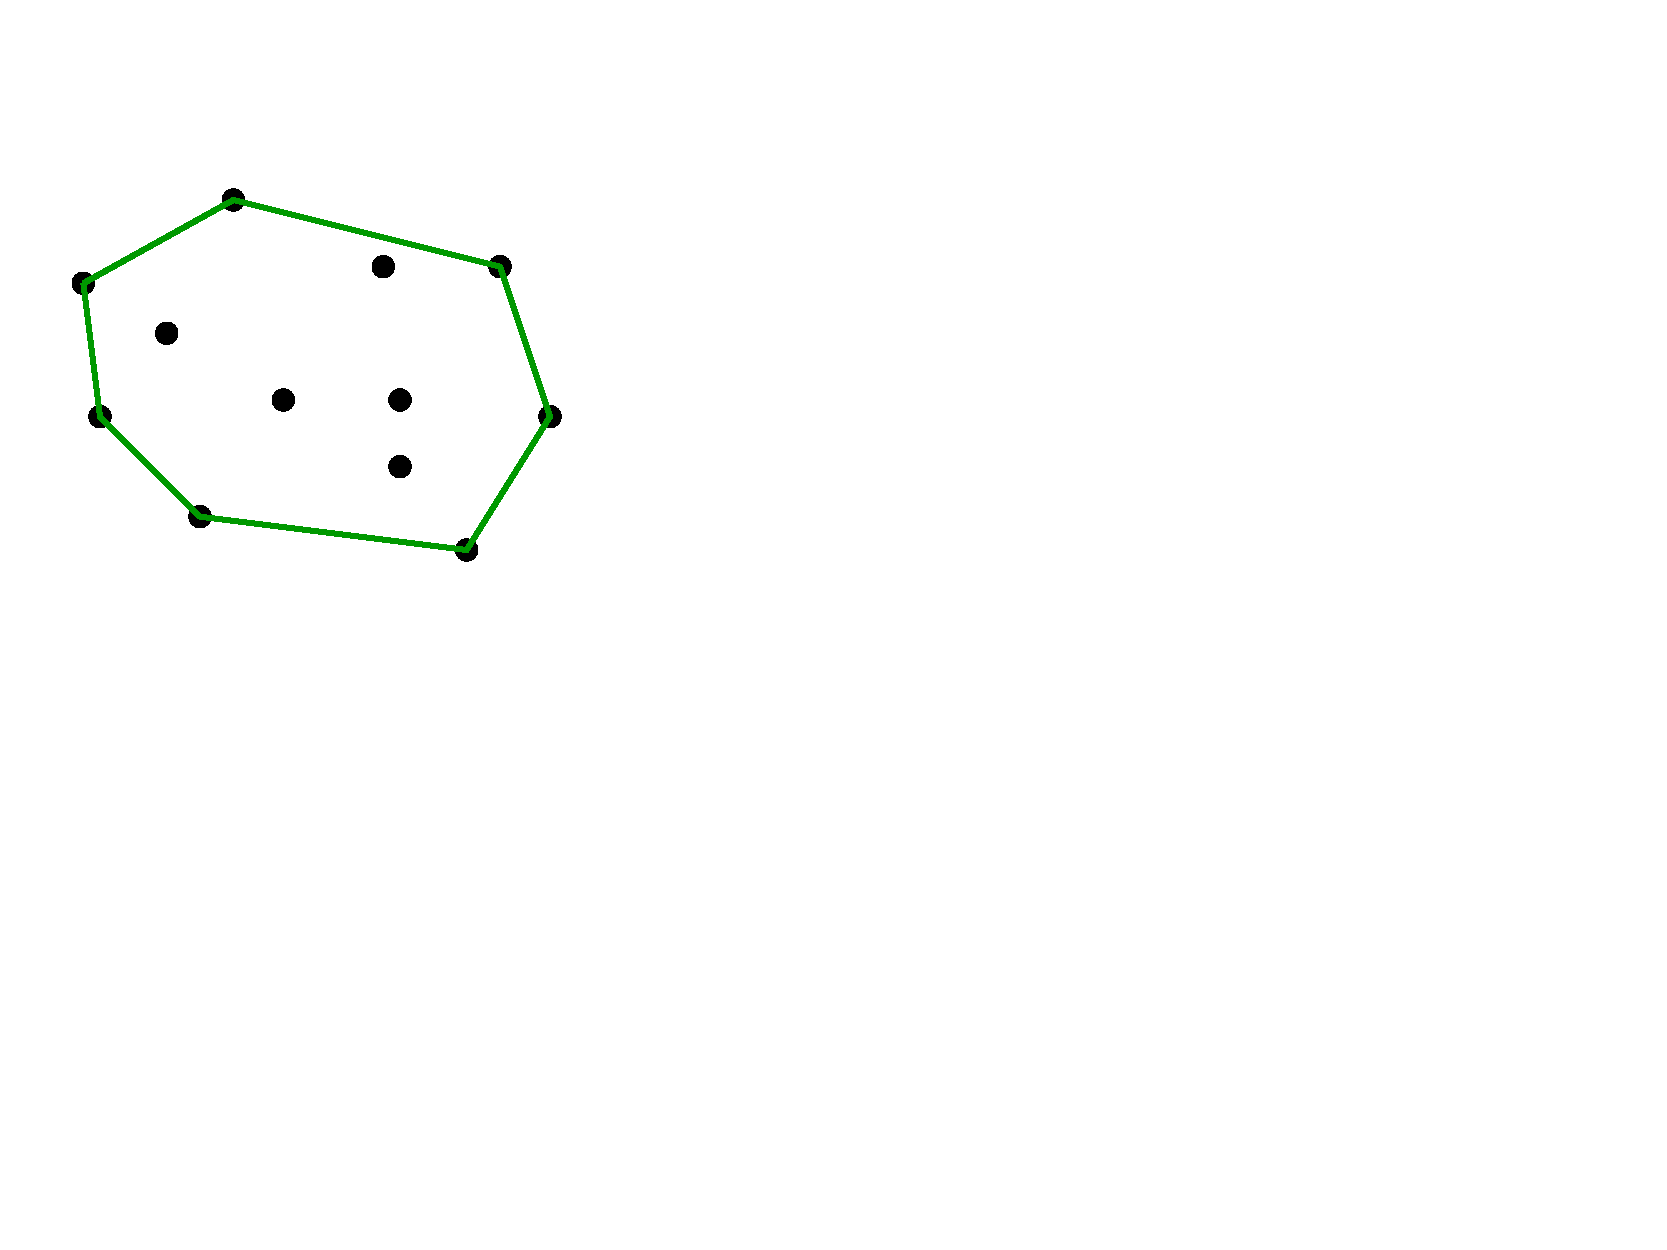
\includegraphics[scale=.75]{convex-2-2}
  \end{overprint}
\end{frame}


\begin{frame}{Course work}

  \begin{tabular}{lll}
    SNo & Code & Course Title\\\hline
    1 & CP7009 & Machine Learning Techniques\\
    2 & SE7003 & Machine Learning\\
    3 & MA7155 & Applied Probability and Statistics \\    
    4 & IF7203 & Data Warehousing and Data Mining \\
    5 & SE7204 & Big Data Analytics\\
    6 & CP7201 & Theoretical Foundations  of Computer Science\\
    7 & CP7024 & Information Retrieval Techniques \\
  \end{tabular} 
\end{frame}

\section{References}

\begin{frame}[allowframebreaks]
  \frametitle<presentation>{Reference}
  \small
  \begin{thebibliography}{10}
    \beamertemplatebookbibitems
  \bibitem{Marjan2009} Marjan Mernik, Dejan Hrncic, Barrett R. Bryant,
    Alan P. Sprague, Jeff Gray, Qichao Liu, Faizan Javed.
    \emph{Grammar Inference Algorithms and Applications in Software
      Engineering}, 978-1-4244-4221-8/09, IEEE, 2009.
  \bibitem{Colin2010} Colin de la Higuera.
    \emph{Grammatical Inference: Learning Automata and Grammars},
    Cambridge University Press, 2010.
 
    \beamertemplatearticlebibitems
    % Followed by interesting articles. Keep the list short.

  \bibitem{Arianna2011} Arianna D'Ulizia, Fernando Ferri, Patrizia
    Grifoni.
    \emph{A survey of grammatical inference methods for natural
      language learning},
    Artificial Intelligence Review, DOI 10.1007/s10462-010-9199-1,
    Springer, January 2011.
  \bibitem{Harald2013} Harald Lampesberger. 
    \emph{A Grammatical Inference Approach to Language-Based Anomaly
      Detection in XML},
    First Int Workshop on Emerging Cyberthreats and Countermeasures,
    Regensburg, Germany, September 2013.
  \end{thebibliography}
\end{frame}

\begin{frame}
  \begin{center}
    Questions?
  \end{center}

  \vfill
  \pause
  \begin{center}
    Thank you!
  \end{center}
\end{frame}
\end{document}
